%
% Copyright (C) 2017 CERN
%
% Author: Marco Guerri
%
% This program is free software: you can redistribute it and/or modify
% it under the terms of the GNU General Public License as published by
% the Free Software Foundation, either version 3 of the License, or
% (at your option) any later version.
%
% This program is distributed in the hope that it will be useful,
% but WITHOUT ANY WARRANTY; without even the implied warranty of
% MERCHANTABILITY or FITNESS FOR A PARTICULAR PURPOSE.  See the
% GNU General Public License for more details.
%
% You should have received a copy of the GNU General Public License
% along with this program.  If not, see <http://www.gnu.org/licenses/>
%
\documentclass[xcolor=table]{beamer}
\usepackage{beamerthemecern}
\usepackage{booktabs}
\usepackage{pgffor}
\usepackage{lstlinebgrd}
\usepackage[export]{adjustbox}
\usepackage{enumitem}
\usepackage{caption}
\usepackage{listings}
\usepackage{tikz}
\usepackage{filecontents}
\usepackage{pgfplots}
\usetikzlibrary{arrows,shapes,calc}

\definecolor{lightblue}{gray}{0.95}

% Customize caption for listing removing "Listing X"
\DeclareCaptionFormat{listing}{\colorbox{lightblue}{\parbox{\textwidth - 2mm}{#3}}}
\captionsetup[lstlisting]{format=listing,font={scriptsize,sf},justification=centering}

% Zebra colored listings
\newcommand\realnumberstyle[1]{}
\makeatletter

% Wider command
\newcommand\Wider[2][3em]{%
\makebox[\linewidth][c]{%
  \begin{minipage}{\dimexpr\textwidth+#1\relax}
  \raggedright#2
  \end{minipage}%
  }%
}

\newcommand{\zebra}[3]{%
    {\realnumberstyle{#3}}%
    \begingroup
    \lst@basicstyle
    \ifodd\value{lstnumber}%
        \color{#1}%
    \else
        \color{#2}%
    \fi
        \rlap{\hspace*{\lst@numbersep}%
        \color@block{\linewidth}{\ht\strutbox}{\dp\strutbox}%
        }%
    \endgroup
}
\makeatother

% Listing customization
\lstset{
    language=Python,                % choose the language of the code
    basicstyle=\fontfamily{pcr}\tiny,       % the size of the fonts that are used for the code
    tabsize=2,
    captionpos=b,
    numbers=left,
    stepnumber=1,
    numberstyle=\tiny,
    numbersep=5pt,
    frame=lines,
    escapeinside={|@}{@|},
    breaklines=true,
    keywordstyle=\color[rgb]{0,0,1},
    commentstyle=\color[rgb]{0.133,0.545,0.133},
    stringstyle=\color[rgb]{1,0,0}
}

\makeatletter


%%%%%%%%%%%%%%%%%%%%%%%%%%%%%%%%%%%%%%%%%%%%%%%%%%%%%%%%%%%%%%%%%%%%%%%%%%%%%%
% tikz tools
%%%%%%%%%%%%%%%%%%%%%%%%%%%%%%%%%%%%%%%%%%%%%%%%%%%%%%%%%%%%%%%%%%%%%%%%%%%%%%
\tikzset{
    invisible/.style={opacity=0},
    visible on/.style={alt={#1{}{invisible}}},
    alt/.code args={<#1>#2#3}{%
      \alt<#1>{\pgfkeysalso{#2}}{\pgfkeysalso{#3}} % \pgfkeysalso doesn't change the path
    },
  }

\newcommand{\tikzmark}[2]{%
     \tikz[overlay,remember picture] \node[text=black,
           inner sep=0pt] (#1) {#2};}

%%%%%%%%%%%%%%%%%%%%%%%%%%%%%%%%%%%%%%%%%%%%%%%%%%%%%%%%%%%%%%%%%%%%%%%%%%%%%%
%
% \btIfInRange{number}{range list}{TRUE}{FALSE}
%
% Test in int number <number> is element of a (comma separated) list of ranges
% (such as: {1,3-5,7,10-12,14}) and processes <TRUE> or <FALSE> respectively
%%%%%%%%%%%%%%%%%%%%%%%%%%%%%%%%%%%%%%%%%%%%%%%%%%%%%%%%%%%%%%%%%%%%%%%%%%%%%%
\newcount\bt@rangea
\newcount\bt@rangeb

\newcommand\btIfInRange[2]{%
    \global\let\bt@inrange\@secondoftwo%
    \edef\bt@rangelist{#2}%
    \foreach \range in \bt@rangelist {%
        \afterassignment\bt@getrangeb%
        \bt@rangea=0\range\relax%
        \pgfmathtruncatemacro\result{ ( #1 >= \bt@rangea) && (#1 <= \bt@rangeb) }%
        \ifnum\result=1\relax%
            \breakforeach%
            \global\let\bt@inrange\@firstoftwo%
        \fi%
    }%
    \bt@inrange%
}
\newcommand\bt@getrangeb{%
    \@ifnextchar\relax%
        {\bt@rangeb=\bt@rangea}%
        {\@getrangeb}%
}
\def\@getrangeb-#1\relax{%
    \ifx\relax#1\relax%
        \bt@rangeb=100000%   \maxdimen is too large for pgfmath
    \else%
        \bt@rangeb=#1\relax%
    \fi%
}

\newcommand<>{\btLstHL}[1]{%
  \only#2{\btIfInRange{\value{lstnumber}}{#1}
        {\color{lightgray}\def\lst@linebackgroundcolor{\color@block}}
        {\def\lst@linebgrdcmd####1####2####3{}}}%
}%
\makeatother

\begin{document}
\title{Understanding applications performance}
\author{Marco Guerri}
\date{\today}

\frontcover
\frame{\titlepage}
\frame{\tableofcontents}

%%%%%%%%%%%%%%%%%%%%%%%%%%%%%%%%%%%%%%%%%%%%%%%%%%%%%%%%%%%%%%%%%%%%%%%%%%%%%%%
% 
% Dirac Benchmark 2012
%
%%%%%%%%%%%%%%%%%%%%%%%%%%%%%%%%%%%%%%%%%%%%%%%%%%%%%%%%%%%%%%%%%%%%%%%%%%%%%%%%
\section{Dirac Benchmark 2012}
\begin{frame}[fragile]{Dirac Benchmark 12}
\vspace{-5mm}
    \begin{columns}[t]
        \begin{column}{0.55\textwidth}
            \setlist{leftmargin=4mm,label=$\diamond$}
            \hypersetup{colorlinks=true, linkbordercolor=red, pdfborderstyle={/S/U/W 0.2}}
            \begin{lstlisting}[language=Python, caption=Excerpt from Dirac Benchmark 12
                                (\href{https://github.com/DIRACGrid/DB12}{github}),
                                 numbers=none]
  for i in range( iterations + 1 ):
    if i == 1:
        start = os.times()
    # Now the iterations
    for j in range( n ):
      t = random.normalvariate( 10, 1 )
      m += t
      m2 += t * t
      p += t
      p2 += t * t

  end = os.times()
  cput = sum( end[:4] ) - sum( start[:4] )
  wall = end[4] - start[4]
            \end{lstlisting}
        \end{column}
    \begin{column}{0.55\textwidth}

\def\arraystretch{1.2}
\arrayrulewidth=0.4pt

\begin{minipage}[t][4cm][t]{\textwidth}
\only<5->{
\vspace{-7mm}
\begin{table}

\def\fourthrowcolor{}
\def\fifthrowcolor{}
\def\sixthrowcolor{}
\def\seventhrowcolor{}
\only<7>{\def\fourthrowcolor{\rowcolor{lightgray}}}
\only<8>{\def\fifthrowcolor{\rowcolor{lightgray}}}
\only<9>{\def\sixthrowcolor{\rowcolor{lightgray}}}
\only<10>{\def\seventhrowcolor{\rowcolor{lightgray}}}

\tiny
\begin{tabular}{ l |  l |  l   }
   \multicolumn{3}{ c }{Hardware configuration} \\
   \hline
   & \textbf{Ivy Bridge} & \textbf{Haswell} \\
  \hline
  CPU & E5-2650v2  & E5-2640v3  \\
  Core/Threads & 8/16 & 8/16  \\
  Base/Turbo CLK & 2.6/3.4  & 2.6/3.4  \\
  RAM  & 64 GiB DDR3 & 128 GiB DDR4 \\
  OS & CentOS 7.3 & CentOS 7.3  \\
  gcc & 4.8.5 & 4.8.5  \\
  Python & 2.7.5-48 & 2.7.5-48 \\
   \hline
   \multicolumn{3}{ c }{Benchmark results} \\
    \hline
    \fourthrowcolor $HS06_{32 t}$ & 350.19 & 360.87 \\
    \fifthrowcolor $HS06_{1 t}$ & 26.35 & 28.54  \\
    \sixthrowcolor $DB12_{32 t}$ & 10.98 & 12.27 \\
    \seventhrowcolor $DB12_{1 t}$ & 20.99 & 30.17 \\ 
    \hline
\end{tabular}
\end{table}
}
\end{minipage}

% Additional step for impressive zoom-in
\only<6>{}


\end{column}
\end{columns}

            \setlist{leftmargin=4mm,label=$\diamond$}
            \begin{itemize}[noitemsep,topsep=0pt]
            \small
                \item<2-> Python benchmark, less than 100 LOC, 2 minutes runtime
                 \item<3-> Iteration over \textit{random.normalvariate()} plus arithmentic operations
                 \item<4-> Considered an excellent predictor of performance of
                          LHCb MC jobs
            \end{itemize}
\end{frame}

\begin{frame}[fragile]{DB 12 - Functions profile}
\begin{lstlisting}[language=Python, caption=Functions profile on Ivy Bridge,
                   linebackgroundcolor={%
                        \btLstHL<2>{2}%
                        \btLstHL<3>{7}}]
#rank % cumulative%  function-name             image-name
0:  40.065  40.065  PyEval_EvalFrameEx        /lib64/libpython2.7.so.1.0
1:  10.345  50.410  _Py_add_one_to_index_C    /lib64/libpython2.7.so.1.0
2:   6.474  56.884  PyFloat_GetInfo           /lib64/libpython2.7.so.1.0
3:   3.743  60.627  _PyLong_Init              /lib64/libpython2.7.so.1.0
4:   3.600  64.227  PyFloat_FromDouble        /lib64/libpython2.7.so.1.0
5:   3.530  67.756  .text                     /usr/lib64/.../_randommodule.so
6:   3.089  70.845  Py_UniversalNewlineFread  /lib64/libpython2.7.so.1.0
7:   2.665  73.510  __ieee754_log_avx         /lib64/libm.so.6
8:   2.554  76.065  PyDict_GetItem            /lib64/libpython2.7.so.1.0
9:   2.273  78.337  _PyFloat_Unpack8          /lib64/libpython2.7.so.1.0
\end{lstlisting}

\vspace{-1mm}
\begin{lstlisting}[language=Python, caption=Functions profile on Haswell,
                   linebackgroundcolor={%
                        \btLstHL<2>{2}%
                        \btLstHL<3>{7}}]
#rank % cumulative%  function-name             image-name
0:  40.061  40.061  PyEval_EvalFrameEx        /lib64/libpython2.7.so.1.0
1:  10.344  50.406  _Py_add_one_to_index_C    /lib64/libpython2.7.so.1.0
2:   6.474  56.879  PyFloat_GetInfo           /lib64/libpython2.7.so.1.0
3:   3.743  60.622  _PyLong_Init              /lib64/libpython2.7.so.1.0
4:   3.599  64.222  PyFloat_FromDouble        /lib64/libpython2.7.so.1.0
5:   3.529  67.751  .text                     /usr/lib64/.../_randommodule.so
6:   3.089  70.840  Py_UniversalNewlineFread  /lib64/libpython2.7.so.1.0
7:   2.665  73.504  __ieee754_log_avx         /lib64/libm.so.6
8:   2.554  76.059  PyDict_GetItem            /lib64/libpython2.7.so.1.0
9:   2.273  78.331  _PyFloat_Unpack8          /lib64/libpython2.7.so.1.0
\end{lstlisting}

\end{frame}

\begin{frame}[t,fragile]
\frametitle{DB 12 - Instructions breakdown}
\begin{minipage}[t][2cm][t]{\textwidth}
\vspace{-0.5cm}
\begin{lstlisting}[language=Python, linebackgroundcolor={%
                                    \btLstHL<2-6>{2}%
                                    \btLstHL<7>{7}%
                                    \btLstHL<8>{9}}]
#rank % cumulative%  function-name             image-name
0:  40.065  40.065  PyEval_EvalFrameEx        /lib64/libpython2.7.so.1.0
1:  10.345  50.410  _Py_add_one_to_index_C    /lib64/libpython2.7.so.1.0
2:   6.474  56.884  PyFloat_GetInfo           /lib64/libpython2.7.so.1.0
3:   3.743  60.627  _PyLong_Init              /lib64/libpython2.7.so.1.0
4:   3.600  64.227  PyFloat_FromDouble        /lib64/libpython2.7.so.1.0
5:   3.530  67.756  .text                     /usr/lib64/.../_randommodule.so
6:   3.089  70.845  Py_UniversalNewlineFread  /lib64/libpython2.7.so.1.0
7:   2.665  73.510  __ieee754_log_avx         /lib64/libm.so.6
\end{lstlisting}
\end{minipage}

\begin{figure}[H]
\begin{center}
\includegraphics[scale=0.23]<2-6>{images/PyEval_EvalFrameEx.png}
\includegraphics[scale=0.23]<7>{images/_randommodule.png}
\includegraphics[scale=0.23]<8>{images/__ieee754_log_avx.png}
\end{center}
\end{figure}
\end{frame}

\begin{frame}[fragile]{DB 12 - PyEval\_EvalFrameEx analysis}
\begin{columns}[t]

\begin{column}{0.5\textwidth}
\vspace{-5mm}
\setlist{leftmargin=1mm,label=$\diamond$}
\begin{itemize}
    \small
    \item Python source code is compiled into bytecode
    \item Bytecode is executed by interpreter (CPython)
\end{itemize}
\begin{lstlisting}[language=Python, caption=Function disassembly,
                   linebackgroundcolor={\btLstHL<2>{1-5}%
                                        \btLstHL<3->{6-17}%
                                        \btLstHL<5>{12}}]
>>> def myfunc():
...     a = 120
...     b = a*10
...     return b
...
>>> import dis
>>> dis.dis(myfunc)
  2           0 LOAD_CONST         1 (120)
              3 STORE_FAST         0 (a)

  3           6 LOAD_FAST          0 (a)
              9 LOAD_CONST         2 (10)
             12 BINARY_MULTIPLY
             13 STORE_FAST         1 (b)

  4          16 LOAD_FAST          1 (b)
             19 RETURN_VALUE
\end{lstlisting}
\end{column}

\begin{column}{0.5\textwidth}<4->
\vspace{-5mm}
\begin{lstlisting}[language=c, caption=Excerpt from PyEval\_EvalFrameEx,
                   linebackgroundcolor={\btLstHL<5->{8}}]
switch (opcode) {
    case NOP:
        <NOP Instruction>
        break;
    case LOAD_FAST:
        <LOAD_FAST Instruction>
        break;
    case LOAD_CONST:
        <LOAD_CONST Instruction>
        break;
    case STORE_FAST:
        <STORE_FAST Instruction>
        break;
    case POP_TOP:
        <POP_TOP Instruction>
        break;
    case ROT_TWO:
        <ROT_TWO Instruction>
        break;
    [...]
    case UNARY_CONVERT:
        <UNARY_CONVERT Instruction>
        break;
    [..]
}
\end{lstlisting}
\end{column}
\end{columns}
\end{frame}

\begin{frame}[fragile]{DB 12 - Profiling}{Only}

\begin{table}
\def\firstrowcolor{}
\def\secondrowcolor{}
\def\thirdrowcolor{}
\def\fourthrowcolor{}
\def\fifthrowcolor{}
\def\sixthrowcolor{}
\def\seventhrowcolor{}
\def\eighthrowcolor{}
\def\ninethrowcolor{}
\def\tenthrowcolor{}
\def\eleventhrowcolor{}
\def\twelvethrowcolor{}
\def\thirteenthrowcolor{}
\def\fourteenthrowcolor{}

\only<2>{\def\firstrowcolor{\rowcolor{lightgray}}}
\only<3>{\def\secondrowcolor{\rowcolor{lightgray}}}
\only<4>{\def\thirdrowcolor{\rowcolor{lightgray}}}
\only<5>{\def\fourthrowcolor{\rowcolor{lightgray}}}
\only<6>{\def\fifthrowcolor{\rowcolor{lightgray}}}
\only<7>{\def\sixthrowcolor{\rowcolor{lightgray}}}
\only<8>{\def\seventhrowcolor{\rowcolor{lightgray}}}
\only<9>{\def\eighthrowcolor{\rowcolor{lightgray}}}
\only<10>{\def\ninethrowcolor{\rowcolor{lightgray}}}
\only<11>{\def\tenthrowcolor{\rowcolor{lightgray}}}
\only<12>{\def\eleventhrowcolor{\rowcolor{lightgray}}}
\only<13>{\def\twelvethrowcolor{\rowcolor{lightgray}}}
\only<14>{\def\thirteenthrowcolor{\rowcolor{lightgray}}}
\only<15>{\def\fourteenthrowcolor{\rowcolor{lightgray}}}
\scriptsize
\begin{tabular}{ l |  r |  r | r }
   \multicolumn{4}{ c }{Performance statistics} \\
   \hline
   & \textbf{Ivy Bridge} & \textbf{Haswell} &  $\Delta$ \\
    \hline
  \firstrowcolor task-clock & 34725.557061  & 24105.686437 &  10s\\
  \secondrowcolor context-switches & 1,757  & 1,220 & -30\% \\
  \thirdrowcolor cpu-migrations & 0  & 1 &  \\
  \fourthrowcolor page-faults & 77,735  & 77,727 &  -0.01\% \\
  \fifthrowcolor cycles & 115,880,566,912  & 79,856,590,321 &  \\
  \sixthrowcolor stalled-cycles-frontend & 33,935,812,197  & -  &  \\
  \seventhrowcolor instructions & 196,423,070,931  & 196,279,702,821 & -0.07\% \\
  \eighthrowcolor branches & 39,007,221,715  & 38,988,806,436 & -0.04\%  \\
  \ninethrowcolor \fourteenthrowcolor branch-misses & 771,858,119  & 148,049,799 & -80\% \\
  \tenthrowcolor L1-dcache-loads & 65,738,912,645  & 65,709,868,550 & -0.4\% \\
  \eleventhrowcolor L1-dcache-load-misses & 223,445,275  & 190,642,933 & -14.6\% \\
  \twelvethrowcolor LLC-loads & 18,182,616  & 17,276,409 & -5\% \\
  \thirteenthrowcolor LLC-load-misses & 12,658,059  & 12,296,728 & -2.8\%  \\
  \hline
\end{tabular}
\end{table}
\setlist{leftmargin=10mm,label=$\diamond$}
\begin{minipage}[t][10mm][t]{\textwidth}
\begin{itemize}
    \small
    % Why the first item is not vertically aligned?
    \item<2|only@2> \vspace{1.01mm} Runtime in milliseconds: 10s difference
    \item<2|only@2> \vspace{1.01mm} Looking for architectural explanation
                                    behind additional speedup
    \item<3|only@3> Context switches most likeley due to timer softirq
    \item<3|only@3> 500 more context switches on Ivy Bridge, cost is negligible
    \item<4|only@4> One more CPU migration on Haswell, cost is negligible
    \item<5|only@5> 8 more page-faults on Ivy Bridge, cost is negligible
    \item<8|only@8> Same number of instructions executed
    \item<9|only@9> Same number of branches
    \item<10|only@10> 623808320 more mispredicted branches on Ivy Bridge
    \item<10|only@10> 20 cycles per mispredicted branch @ ~3.4GHz = 4s
    \item<11|only@11> Negligible difference in L1d loads
    \item<12|only@12> 32802342 more misses on Ivy Bridge
    \item<12|only@12> 10 cycles per L1 miss, assuming it hits L2 = \textless 1s
\end{itemize}
\end{minipage}
% Ivy Bridge Profile
%      34725.557061      task-clock (msec)         #    1.000 CPUs utilized
%             1,757      context-switches          #    0.051 K/sec
%                 0      cpu-migrations            #    0.000 K/sec
%            77,735      page-faults               #    0.002 M/sec
%   115,880,566,912      cycles                    #    3.337 GHz                      (44.45%)
%    33,935,812,197      stalled-cycles-frontend   #   29.29% frontend cycles idle     (44.45%)
%   196,423,070,931      instructions              #    1.70  insn per cycle
%                                                  #    0.17  stalled cycles per insn  (55.56%)
%    39,007,221,715      branches                  # 1123.300 M/sec                    (55.56%)
%       771,858,119      branch-misses             #    1.98% of all branches          (55.56%)
%    65,738,912,645      L1-dcache-loads           # 1893.099 M/sec                    (44.44%)
%       223,445,275      L1-dcache-load-misses     #    0.34% of all L1-dcache hits    (22.22%)
%        18,182,616      LLC-loads                 #    0.524 M/sec                    (22.22%)
%        12,658,059      LLC-load-misses           #   69.62% of all LL-cache hits     (33.33%)
%      34.734003622 seconds time elapsed

% Haswell profile
%      24105.686437      task-clock (msec)         #    1.000 CPUs utilized
%             1,220      context-switches          #    0.051 K/sec
%                 1      cpu-migrations            #    0.000 K/sec
%            77,727      page-faults               #    0.003 M/sec
%    79,856,590,321      cycles                    #    3.313 GHz                      (50.00%)
%   196,279,702,821      instructions              #    2.46  insn per cycle           (62.50%)
%    38,988,806,436      branches                  # 1617.411 M/sec                    (62.51%)
%       148,049,799      branch-misses             #    0.38% of all branches          (62.51%)
%    65,709,868,550      L1-dcache-loads           # 2725.907 M/sec                    (62.50%)
%       190,642,933      L1-dcache-load-misses     #    0.29% of all L1-dcache hits    (25.00%)
%        17,276,409      LLC-loads                 #    0.717 M/sec                    (24.99%)
%        12,296,728      LLC-load-misses           #   71.18% of all LL-cache hits     (37.50%)
%
%      24.117095520 seconds time elapsed


\end{frame}
\begin{frame}[fragile]{DB 12 - Mispredicted branches (CC7)}

\setlist{leftmargin=1mm,label=$\diamond$}
\begin{lstlisting}[language=Python, caption=Mispredicted branches on Ivy Bridge - function annotation (CC7),
                   linebackgroundcolor={\btLstHL<2->{3}}]
Samples: 142K of event 'branch-misses:pp', Event count (approx.): 889919468
Overhead  Command  Shared Object        Symbol
  88.53%  python   libpython2.7.so.1.0  [.] PyEval_EvalFrameEx
   5.81%  python   libpython2.7.so.1.0  [.] 0x00000000000477da
   4.27%  python   libm-2.17.so         [.] __ieee754_log_avx
   1.09%  python   libpython2.7.so.1.0  [.] PyBool_FromLong
   0.03%  python   libpython2.7.so.1.0  [.] PyInt_FromLong
\end{lstlisting}

\vspace{-5mm}
\begin{columns}[t]
\begin{column}{0.45\textwidth}<3->
\begin{lstlisting}[language=Python, caption=Assembly annotation on Ivy Bridge,
                   linebackgroundcolor={\btLstHL<4->{4}}]
          xor    %ecx,%ecx
          mov    %rdx,%rbp
          mov    (%rsi,%rdi,8),%rsi
 45.25%   jmpq   fffffffffff22300
          lea    0x2(%r9),%rbx
          movzbl -0x1(%rbx),%eax
          movzbl -0x2(%rbx),%ecx
\end{lstlisting}
\end{column}
\begin{column}{0.6\textwidth}<6->
\begin{lstlisting}[language=Python, caption=Corresponding C code,
                   linebackgroundcolor={\btLstHL<7->{4}}]
#define FAST_DISPATCH() { \
    if (!_Py_TracingPossible) { \
        f->f_lasti = INSTR_OFFSET(); \
        goto *opcode_targets[*next_instr++]; \
    } \
    goto fast_next_opcode;\
}
\end{lstlisting}

\end{column}
\end{columns}
\begin{itemize}
    \footnotesize
    \item<5-> Actually a \textbf{jmp *rsi}
    \item<8-> Dispatches next opcode to corresponding case branch without \textit{continue}. Other branch mispredictions are on the same FAST\_DISPATCH() macro.
\end{itemize}
\end{frame}

%%%%%%%%%%%%%%%%%%%%%%%%%%%%%%%%%%%%%%%%%%%%%%%%%%%%%%%%%%%%%%%%%%%%%%%%%%%%%%%
% Mispredicted branches on SLC6
%%%%%%%%%%%%%%%%%%%%%%%%%%%%%%%%%%%%%%%%%%%%%%%%%%%%%%%%%%%%%%%%%%%%%%%%%%%%%%%%
\begin{frame}[fragile]{DB 12 - Mispredicted branches (SLC6)}
\setlist{leftmargin=1mm,label=$\diamond$}
\begin{lstlisting}[language=Python, caption=Mispredicted branches on Ivy Bridge - function annotation,
                   linebackgroundcolor={\btLstHL<2->{3}}]
Samples: 289K of event 'branch-misses:pp', Event count (approx.): 1276562725
Overhead  Command  Shared Object        Symbol
  84.30%  python   libpython2.6.so.1.0  [.] PyEval_EvalFrameEx
   4.06%  python   libpython2.6.so.1.0  [.] 0x0000000000045510
   3.25%  python   libm-2.12.so         [.] __ieee754_log
\end{lstlisting}
\setlist{leftmargin=1mm,label=$\diamond$}
\vspace{-5mm}
\begin{columns}[t]
\begin{column}{0.6\textwidth}
\begin{lstlisting}[language=Python, caption=Assembly annotation on Ivy Bridge (SLC6),
                   linebackgroundcolor={\btLstHL<3->{4}}]
        mov    %r8d,%eax
        movslq (%rsi,%rax,4),%rax
        add    %rsi,%rax
 97.40  jmpq   ffffffca30b2f870
        nop
        cmpb   $0x7a,(%r14)
        je     366
\end{lstlisting}
\begin{itemize}
    \footnotesize
    \item<4-> Again indirect jump \textbf{jmp *rax}
    \item<6-> FAST\_DISPATCH() not supported in Python 2.6.6, all
    mispredictions happen on switch statement
\end{itemize}
\end{column}
\begin{column}{0.4\textwidth}
\begin{lstlisting}[language=c, caption=Corresponding C code,
                   linebackgroundcolor={\btLstHL<5->{4}}]
/* Main switch on opcode */
READ_TIMESTAMP(inst0);

switch (opcode) {

    case NOP:
        goto fast_next_opcode;

    case LOAD_FAST:
        x = GETLOCAL(oparg);
        if (x != NULL) {
            Py_INCREF(x);
            PUSH(x);
            goto fast_next_opcode;
        }
\end{lstlisting}

\end{column}
\end{columns}
\end{frame}

%%%%%%%%%%%%%%%%%%%%%%%%%%%%%%%%%%%%%%%%%%%%%%%%%%%%%%%%%%%%%%%%%%%%%%%%%%%%%%%
% What is the difference?
%%%%%%%%%%%%%%%%%%%%%%%%%%%%%%%%%%%%%%%%%%%%%%%%%%%%%%%%%%%%%%%%%%%%%%%%%%%%%%%%
\begin{frame}[fragile]{DB 12 - switch vs computed gotos}
\setlist{leftmargin=1mm,label=$\diamond$}
\vspace{-5mm}
\begin{columns}[t]
\begin{column}{0.5\textwidth}
\begin{lstlisting}[language=c, caption=switch based implementation SLC6,
                   linebackgroundcolor={\btLstHL<2->{3}},
                    basicstyle=\fontfamily{pcr}\tiny]
fast_next_opcode:
    [...]
  switch (opcode) {

        case NOP:
            goto fast_next_opcode;

        [...]

        case LOAD_CONST:
            x = GETITEM(consts, oparg);
            Py_INCREF(x);
            PUSH(x);
            goto fast_next_opcode;

        PREDICTED_WITH_ARG(STORE_FAST);
        case STORE_FAST:
            v = POP();
            SETLOCAL(oparg, v);
            goto fast_next_opcode;
        [...]
    }
\end{lstlisting}

\end{column}
\begin{column}{0.5\textwidth}

\begin{lstlisting}[language=c, caption=computed gotos implementation - CC7,
                   linebackgroundcolor={\btLstHL<2->{5,14,22}}]
  switch (opcode) {

        TARGET_NOARG(NOP)
        {
            FAST_DISPATCH();
        }

        [...]
        TARGET(LOAD_CONST)
        {
            x = GETITEM(consts, oparg);
            Py_INCREF(x);
            PUSH(x);
            FAST_DISPATCH();
        }

        PREDICTED_WITH_ARG(STORE_FAST);
        TARGET(STORE_FAST)
        {
            v = POP();
            SETLOCAL(oparg, v);
            FAST_DISPATCH();
        }
        [...]
  }
\end{lstlisting}
\end{column}
\end{columns}
\end{frame}
%%%%%%%%%%%%%%%%%%%%%%%%%%%%%%%%%%%%%%%%%%%%%%%%%%%%%%%%%%%%%%%%%%%%%%%%%%%%%%%
% Reproducing mispredicted branches
%%%%%%%%%%%%%%%%%%%%%%%%%%%%%%%%%%%%%%%%%%%%%%%%%%%%%%%%%%%%%%%%%%%%%%%%%%%%%%%%
\begin{frame}[fragile]{DB 12 - Synthetic benchmark}
\setlist{leftmargin=1mm,label=$\diamond$}
\vspace{-5mm}
\begin{columns}[t]
\begin{column}{0.6\textwidth}
\begin{lstlisting}[language=Python, caption=Synthetitc benchmark - indirect branch prediction,
                   linebackgroundcolor={\btLstHL<2>{1-16}%
                                        \btLstHL<3->{18-25}}]
#define CASE(N) \
            case N: \
                fib_n = fib_1 + fib_2; \
                fib_2 = fib_1; \
                fib_1 = fib_n; \
                break;
#define CASE2(N) \
            CASE(N) \
            CASE(N+1)
#define CASE4(N) \
            CASE2(N) \
            CASE2(N+2)
[...]
#define CASE4096(N) \
            CASE2048(N) \
            CASE2048(N+2048)
[...]
while(1) {
    if (i > 0x2FFFFFFF) break;
    opcode = sequence[i % sequence_len];
    switch(opcode) {
        CASE4096(0)
    }
    i++;
}
\end{lstlisting}
\end{column}
\begin{column}{0.4\textwidth}
\begin{lstlisting}[language=c, caption=Sequential vs Random opcode, numbers=none]
|@\tikzmark{one}{}@|case1:
    [...]
    break;
|@\tikzmark{two}{}@|case2:|@\tikzmark{two_right}{}@|
    [...]
    break;
|@\tikzmark{three}{}@|case3:|@\tikzmark{three_right}{}@|
    [...]
    break;
|@\tikzmark{four}{}@|case4:|@\tikzmark{four_right}{}@|
    [...]
    break;
|@\tikzmark{five}{}@|case5:|@\tikzmark{five_right}{}@|
    [...]
    break;
|@
\begin{tikzpicture}[overlay,remember picture]
    \onslide<4-7>{\draw[-stealth, thick, red] (one) to [bend right=70] (two);}
    \onslide<5-7>{\draw[-stealth, thick, red] (two) to [bend right=70] (three);}
    \onslide<6-7>{\draw[-stealth, thick, red] (three) to [bend right=70] (four);}
    \onslide<7>{\draw[-stealth, thick, red] (four) to [bend right=70] (five);}
    \onslide<8->{\draw[-stealth, thick, blue] (one) to [bend right=30] (five);}
    \onslide<9->{\draw[-stealth, thick, blue] (five_right) to [bend right=30] (three_right);}
    \onslide<10->{\draw[-stealth, thick, blue] (three) to [bend left=30] (two);}
    \onslide<11->{\draw[-stealth, thick, blue] (two_right) to [bend left=30] (four_right);}
\end{tikzpicture}
 @|
\end{lstlisting}

\onslide<12->{\footnotesize Random, sequence len 256}
\begin{itemize}
    \footnotesize
    \item<13-> Ivy Bridge: 11.3s, 10\% misses
    \item<14-> Haswell: 4.5s, 0.0\% misses
\end{itemize}
\end{column}
\end{columns}
\end{frame}

%%%%%%%%%%%%%%%%%%%%%%%%%%%%%%%%%%%%%%%%%%%%%%%%%%%%%%%%%%%%%%%%%%%%%%%%%%%%%%%
% Branch prediction mechanisms
%%%%%%%%%%%%%%%%%%%%%%%%%%%%%%%%%%%%%%%%%%%%%%%%%%%%%%%%%%%%%%%%%%%%%%%%%%%%%%%%
\begin{frame}[fragile]{DB 12 - Branch prediction perf}
\pgfplotsset{xlabel style={font=\scriptsize},
             ylabel style={font=\scriptsize},
             yticklabel style={font=\tiny},
             xticklabel style={font=\tiny,rotate=0},
             legend style={at={(0.98,0.3)}, font=\sffamily\tiny},
             grid style={dash pattern = on 0.1mm off 0.5mm,gray}
}
\pgfplotstableread{branch_random_haswell.data}{\pistonkinetics}
\pgfplotstableread{branch_sequential_haswell.data}{\pistonkinetics}
\pgfplotstableread{branch_random_ivybridge.data}{\pistonkinetics}
\pgfplotstableread{branch_sequential_ivybridge.data}{\pistonkinetics}
\begin{center}
\begin{tikzpicture}[scale=1]

\begin{axis}[xtick={0,256,512,1024,2048},
             grid=both,minor tick num=1,
             ylabel=Misprediction rate (\%),
             xlabel=Opcode sequence length,
              legend entries={Haswell random, Haswell sequential, Ivy Bridge random, Ivy Bridge sequential}]

\addplot [blue, thin, fill opacity=0.2,visible on=<2->] table [x={len}, y={mispredictions_random_haswell}] {\pistonkinetics};
\addplot [red, thin, fill opacity=0.2,visible on=<5->] table [x={len}, y={mispredictions_sequential_haswell}] {\pistonkinetics};
\addplot [black, thin, fill opacity=0.2,visible on=<8->] table [x={len}, y={mispredictions_random_ivybridge}] {\pistonkinetics};
\addplot [green, thin, fill opacity=0.2,visible on=<9->] table [x={len}, y={mispredictions_sequential_ivybridge}] {\pistonkinetics};

\node[anchor=west] (source) at (axis cs:256,3.5){};
\node[anchor=west] (source2) at (axis cs:150,3.5){};
\node[anchor=west] (source3) at (axis cs:200,3.5){};
\node[anchor=west] (source4) at (axis cs:900,16){};
\node[anchor=west] (source5) at (axis cs:900,23){};

\node (destination) at (axis cs:512,0.5){};
\node (destination2) at (axis cs:360,0.3){};
\node (destination3) at (axis cs:300,0.4){};
\node (destination4) at (axis cs:1024,13){};
\node (destination5) at (axis cs:1024,19.5){};

\only<3>{\draw[-stealth, thick, blue] (source)--(destination);}
\only<4>{\draw[-stealth, thick, blue] (source)--(destination2);}
\only<6>{\draw[-stealth, thick, red] (source2)--(destination3);}
\only<7>{\draw[-stealth, thick, red] (source4)--(destination4);}
\only<10>{\draw[-stealth, thick, green] (source5)--(destination5);}

\end{axis}
\end{tikzpicture}
\end{center}
\end{frame}
%%%%%%%%%%%%%%%%%%%%%%%%%%%%%%%%%%%%%%%%%%%%%%%%%%%%%%%%%%%%%%%%%%%%%%%%%%%%%%%
% 
% ATLAS Kit Validation
%
%%%%%%%%%%%%%%%%%%%%%%%%%%%%%%%%%%%%%%%%%%%%%%%%%%%%%%%%%%%%%%%%%%%%%%%%%%%%%%%%
\section{ATLAS Kit Validation}
\begin{frame}[fragile]{ATLAS Kit Validation}
\vspace{-20mm}

    \begin{columns}[t]
        \begin{column}{0.55\textwidth}
        \begin{minipage}[t][4cm][t]{\textwidth}
        \small
        \setlist{leftmargin=4mm,label=$\diamond$}
        \begin{itemize}
            \item<1-> Toolkit adopted by the ATLAS collaboration for the validation of their software installation
            \item<1-> Fast benchmark candidate using the GEANT4 simulation of the ATLAS detector
            \item<1-> Simulates $n$ muon particles propagating through the ATLAS
            detector, calculates average simulation time (excluding setup overhead)

            \item<1-> Extensively tested on VMs running on Haswell hypervisors a
                      as part of cloud benchmarking activities [REFERENCE here]
        \end{itemize}
        \end{minipage}
        \end{column}
        \small
        \setlist{leftmargin=4mm,label=$\diamond$}
        \begin{column}{0.50\textwidth}
        \begin{minipage}[t][4cm][t]{\textwidth}
        \begin{figure}[H]
        \begin{center}
            \includegraphics[scale=0.3]<3->{images/dual-mode-gaussian.png}
        \end{center}
        \end{figure}
        \vspace{-7mm}
        \small
        \setlist{leftmargin=4mm,label=$\diamond$}
        \begin{itemize}
            \item<4-> Results highlighted a dual mode gaussian distribution 
            \item<5-> $\Delta mean = 2\%$
            \item<6->\textbf{Effect appearing only with \newline ATLAS KV}
        \end{itemize}
        \end{minipage}
        \end{column}

    \end{columns}

\end{frame}


\begin{frame}[fragile]{Meet ATLAS Kit Validation}

\vspace{-20mm}
\begin{columns}[t]
\begin{column}{0.40\textwidth}
\begin{minipage}[t][4cm][t]{\textwidth}
\begin{lstlisting}[language=Python, caption=/proc/\$(pgrep athena)/status,
                   numbers=none,
                   linebackgroundcolor={%
                   \btLstHL<2>{4,5}%
                   \btLstHL<3>{9}%
                   \btLstHL<4>{13}%
                   \btLstHL<5>{16}%
                   \btLstHL<6>{19}}]
Name:   athena.py
State:  R (running)
[...]
VmPeak:  1389268 kB
VmSize:  1389268 kB
VmLck:         0 kB
VmPin:         0 kB
VmHWM:    973836 kB
VmRSS:    973836 kB
RssAnon:          841472 kB
RssFile:          132364 kB
RssShmem:              0 kB
VmData:   898668 kB
VmStk:       432 kB
VmExe:      1400 kB
VmLib:    215972 kB
VmPTE:      2596 kB
VmSwap:        0 kB
Threads:        2
[...]
\end{lstlisting}
\end{minipage}
\end{column}
\begin{column}{0.70\textwidth}
\begin{minipage}[t][4cm][t]{\textwidth}
\small
\setlist{leftmargin=4mm,label=$\diamond$}
\begin{itemize}
    \item<2-6> Large VA space
    \item<3-6> Large portion or VA space also resident
    \item<4-6> Mostly data (detector geometry, list of particles, properties of the
materials)
    \item<5-6> Large code segment (\textgreater 300 shared objects mapped in the VA space)
    \item<6> Single threaded (plus an additional control thread)

\end{itemize}
\end{minipage}
\end{column}
\end{columns}
\end{frame}

\begin{frame}[t]{ATLAS KV - Bare metal results}
    \begin{columns}[t]
        \begin{column}{1\textwidth}
        \begin{minipage}[t][4cm][t]{\textwidth}
        \vspace{-5mm}
        \begin{figure}[H]
        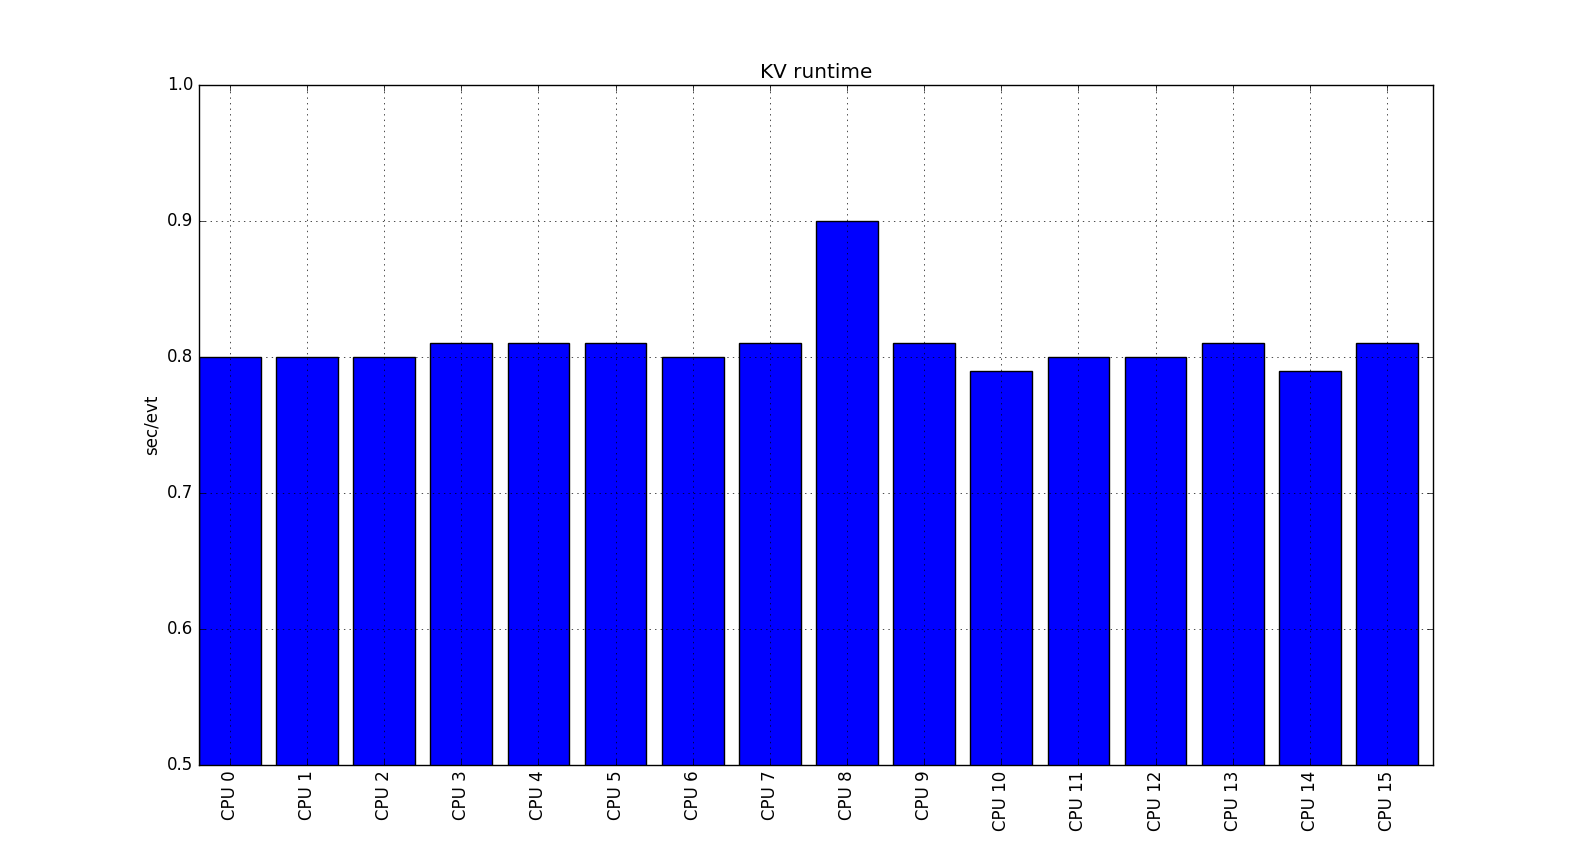
\includegraphics[scale=0.19]{images/kv_runtime.png}
        \end{figure}
        \small
        \setlist{leftmargin=4mm,label=$\diamond$}
        \begin{itemize}
            \item<2-> Single threaded bare metal runs were 12\% slower on CPU 8 (or 8 and 24 with HyperThreading on)
            \item<3-> Some events required up to 20\% more time to be simulated on CPU 8 
            \item<4-> Reproducible in virtualized environment, where single threaded runs were  16\% slower on CPU 8
        \end{itemize}
        \end{minipage}
        \end{column}
    \end{columns}
\end{frame}
\backcover

\end{document}

